\chapter{Evaluation}
\label{eval}
\label{chp:evaluation}
This chapter describes the experiment setup based on the methodology provided in Chapter \ref{chp:methodology}. Following this, the results from the experiment are presented, after which a discussion ensues. The chapter is structured as follows: \S\ref{sec:eval-experiment} describes the hardware used in the experiment, to allow the setup to be reproduced by other researchers. \S\ref{sec:eval-demographic} gives the results of the demographics of the participants taking part in the experiment. In \S\ref{sec:eval-distTests}, the data gathered is presented, together with statistical tests on the two distributions (control and feedback/experiment). \S\ref{sec:eval-ExperimentsResults} highlights the statistically significant differences between the two groups, which may have been caused by the addition of feedback for one group. \S\ref{sec:eval-usersFeedback} presents the results of the second questionnaire, where user feedback and impressions on the systems where gathered. Finally, the chapter closes with a discussion on the results of this study, in \S\ref{sec:eval-Discussion}.

%This chapter provides an insight into the data collected from the questionnaires and \methodname system logs while also explaining results derived from statistical tests. The chapter is structured as follows: \S\ref{sec:eval-experiment} gives an overview of the hardware used. \S\ref{sec:eval-demographic} provides an over of the demographic background for the sampled participants. \S\ref{sec:eval-distTests} covers test which check the data sets distribution moving on to compare the distribution across the feedback group and control group. \S\ref{sec:eval-ExperimentsResults} goes through determining any difference between the two groups which might have been cuased by the introduction of the feedback system. \S\ref{sec:eval-usersFeedback} covers the participants impressions on the experiment and finally conclusive results from this study are presented in \S\ref{sec:eval-Discussion} 

\section{Experiment Setup}
\label{sec:eval-experiment}
The user study has been carried out in line with the methodology described in  
Chapter \ref{chp:methodology}. The sim racing rig framework was custom-built, and the Logitech G25 input devices mounted on it. The display device used was a 32" LCD Samsung monitor capable of outputting HD video resolutions ($1920 \times 1080$) at 60Hz; the chosen display is also capable of outputting stereo audio from 2x10W speakers. The racing simulator used in this experiment is Assetto Corsa by Kunos Simulazioni, running in full HD resolution at 60 frames per second (fps). The hardware platform running the simulator is an Intel Core i7-940, with 8GB of RAM and an Nvidia 660Ti video card with 2GB VRAM. The machine is running the retail version of the Windows 10 Professional operating system.

\begin{figure}
	\centering
	\begin{minipage}{0.45\textwidth}
		\centering
		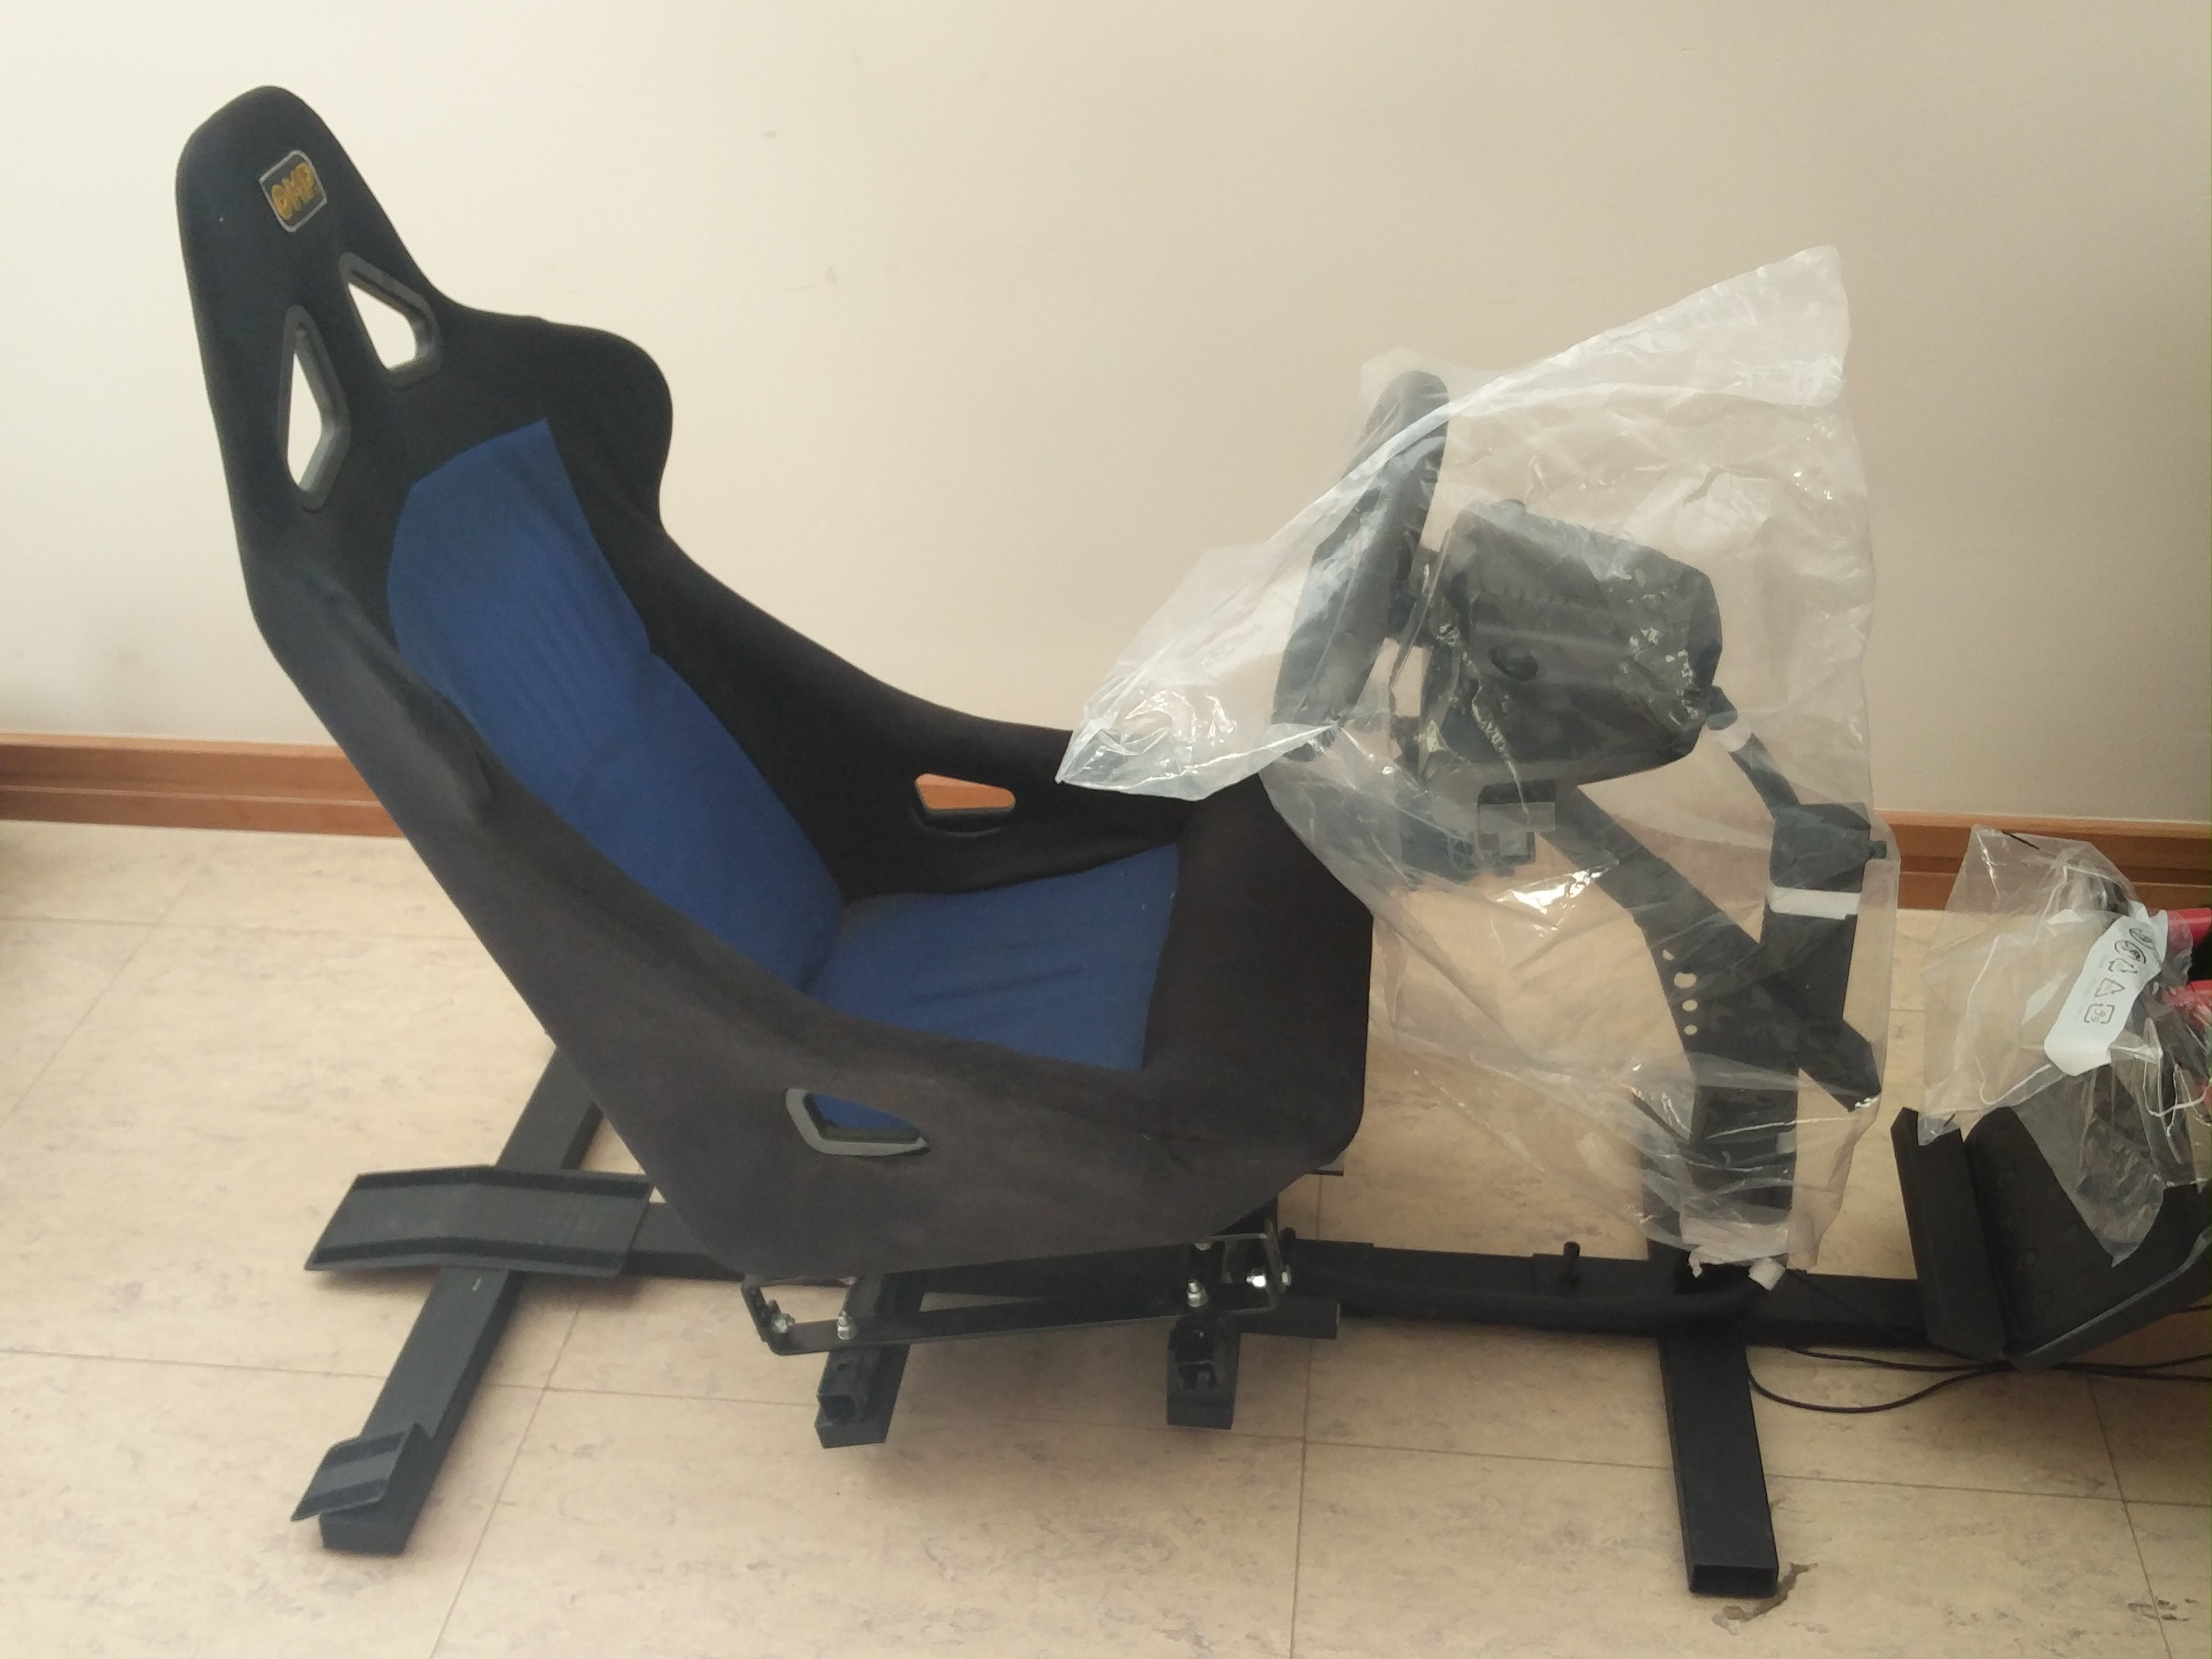
\includegraphics[width=\textwidth]{images/RacingRig}
	\end{minipage}\hfill
	\begin{minipage}{0.45\textwidth}
		\centering
		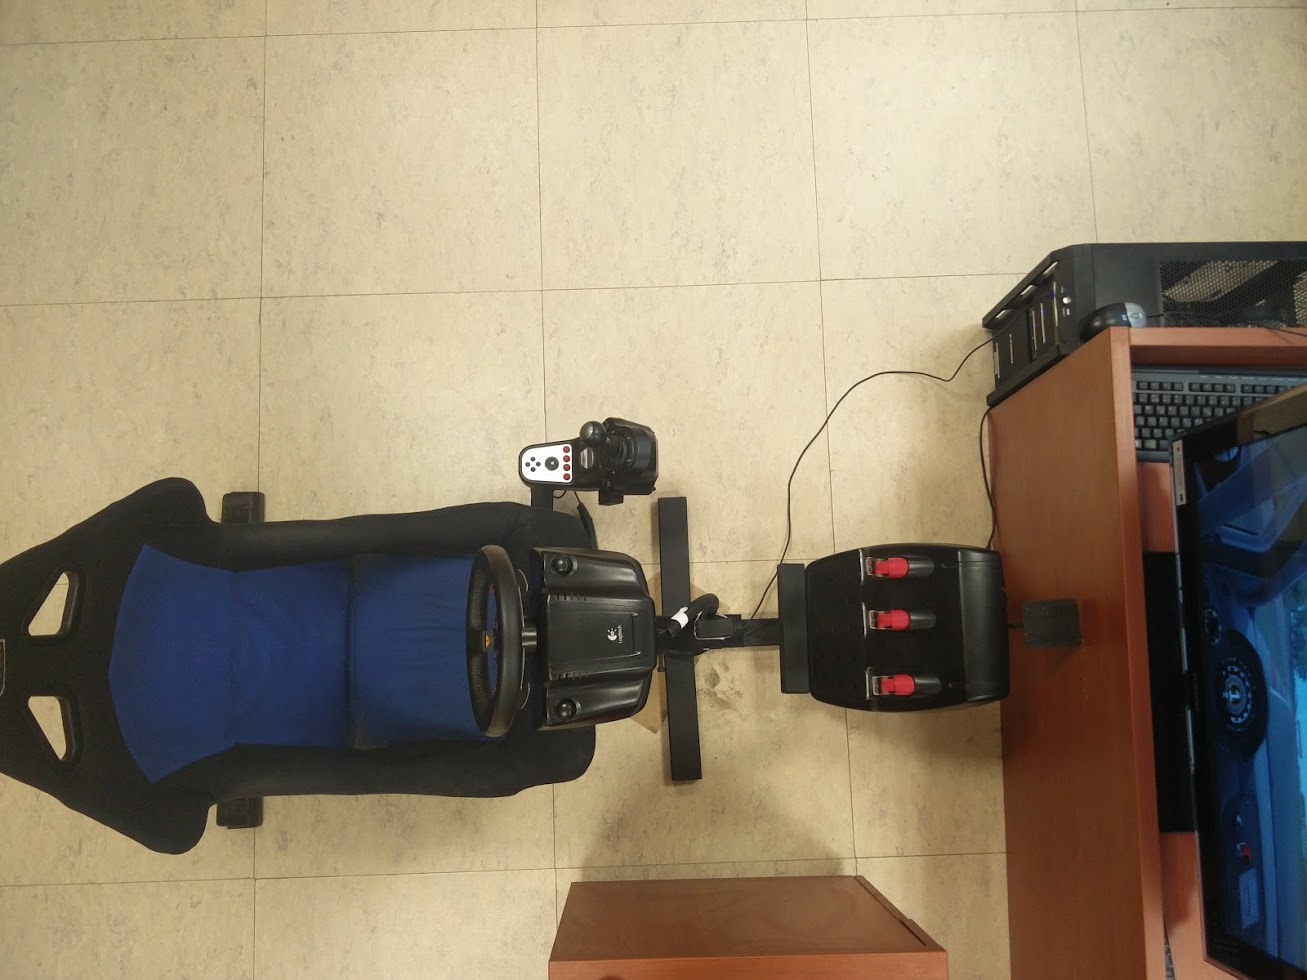
\includegraphics[width=\textwidth]{images/RacingRig2}
	\end{minipage}
	\caption[Side and top view of the racing rig]{Side and top view of the racing rig}
	\label{sec:eval-simRacingRig}
\end{figure}

\section{Sample Demographic}
\label{sec:eval-demographic}
The $1^{st}$ questionnaire, which dealt with participant demographics, showed that most participants were males in their early twenties (see Figure \ref{fig:chart-genderage}). Out of 27 participants, 2 did not hold a driving license; 25 had a driving license, although most of them haven't been driving for more than a year (see Figure \ref{fig:chart-licenseddriversexperience}). 22 participants claimed to play video games (see Figure \ref{fig:chart-playVideoGames}), from which 18 stated to have played racing video games. Out of these 18, a majority of 15 play mostly arcade sim racing games, while the remaining 3 regularly play simulation racing games (see Figure \ref{fig:chart-gamesGenrePlayed}). 7 out of 27 participants have previously used a racing rig (see Figure \ref{fig:chart-usedARacingRig}). Random assignment was used to split the participants into the control and feedback/experimental group. The control group had 13 participants, while the feedback ground had 14.

%didn't add another pie chart as I feel they aren't adding much, but if you think it would help, I can add it

\section{Distribution Tests}
\label{sec:eval-distTests}
This section shows the results of the distribution tests carried out on the gathered data. The histograms for the datasets used are shown in Figure \ref{fig:hist-1}.

\begin{figure}[!htb]
	\centering
	\includegraphics[width=\textwidth]{charts/laptimes.png}
	\caption[Lap times vs session, clustered by group]{Blue : Control Group, Green : Feedback group \\ Lap times vs session, clustered by group}
	\label{fig:chart-laptimes}
\end{figure}

In Figure \ref{fig:chart-laptimes}, a trend appears in which lap times improve as the session progresses, irrespective of the group assignment. The median of the feedback group is lower than that of the control group, except for the final session, where there is less variance in the medians. The participants in the feedback group are less consistent in their lap times, as the whiskers and quartiles in \ref{fig:chart-laptimes} are further spread out when compared to the control group.
%
%one can notice a trend in which lap times improve the more time participants use the rig, irrespective of the group assignment. It's worth pointing out the median of the feedback group is lower than the control group's median, except during the last session in which the medians are close to each other. Moreover the participants in the feedback group seem to be less consistent in their lap times as the box plot whiskers and quartiles are further spread out than the ones from the control group.

The Shapiro-Wilk Test for normality has been carried out on both groups. The dataset employed was that covering the lap times during the first session. The results are shown in Table \ref{table:shapiroWilk}. The p-value for the control group was found to be 0.013, while the feedback group had a p-value of 0.02. Both groups having a p-value lower than 0.05, it can be claimed that the Shapiro-Wilk Test alternative hypothesis is accepted and the samples do not come from a normally distributed dataset.
%With both having a p-value lower than 0.05, the Shapiro-Wilk Test alternative hypothesis is accepted which states the samples do not come from a normally distributed dataset.

\begin{table}[]
	\centering
	\begin{tabular}{ll|rrr|}
		\cline{3-5}
		&                         & \multicolumn{3}{c|}{\textbf{Shapiro-Wilk}}                          \\ \cline{2-2}
		\multicolumn{1}{l|}{\textbf{}}                          & \textbf{Group}          & \textbf{Statistic}        & \textbf{df}             & \textbf{Sig.} \\ \hline
		\multicolumn{1}{|c|}{\multirow{2}{*}{\textbf{LapTime}}} & \textbf{Control Group}  & \multicolumn{1}{r|}{.955} & \multicolumn{1}{r|}{70} & .013          \\ \cline{2-5} 
		\multicolumn{1}{|c|}{}                                  & \textbf{Feedback Group} & \multicolumn{1}{r|}{.963} & \multicolumn{1}{r|}{81} & .020          \\ \hline
	\end{tabular}
	\caption[Shapiro Wilk Test results]{Shapiro Wilk Test results}
	\label{table:shapiroWilk}
\end{table}

The same dataset was subjected to the Kolmogorov-Smirnov Test; the results are shown in Figure \ref{fig:chart-KolmogorowSmimov}. With a significance level of 0.05 and a result having a p-value of 0.360 the null hypothesis is accepted. The groups share the same distribution.

\begin{figure}[!htb]
	\centering
	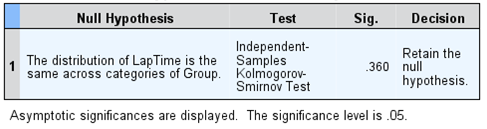
\includegraphics[width=\textwidth]{images/KolmogorowSmimov.png}
	\caption[Kolmogorow Smimov Test]{Kolmogorow Smimov test result}
	\label{fig:chart-KolmogorowSmimov}
\end{figure}

\section{Experiments Results}
\label{sec:eval-ExperimentsResults}
The histograms for the datasets using in the following tests are shown in figures \ref{fig:hist-1}, \ref{fig:hist-2}, \ref{fig:hist-3} and \ref{fig:hist-4}.

Having established that the first session lap times for both groups share the same distribution, the Mann-Whitney Test is used to determine differences in the groups prior to the introduction of feedback in the feedback group. The results of the test are shown in Table \ref{table:Mann-Whitney}. These show a p-value of 0.057 with a confidence interval of 0.95 resulting in no statistical difference between the groups (p-value $> 0.05$, thus accepting the alternative hypothesis). 

%Having established both groups' lap times share the same distribution during the first session, the Mann-Whitney Test is used to determine if any differences between the groups exist before \methodname is introduced to the feedback group. The results of the test are shown in Table \ref{table:Mann-Whitney}. These show a p-value of 0.057 with a confidence interval of 0.95 resulting in no statistical difference between the groups at the start of the sessions as the p-value is greater than 0.05, accepting the alternative hypothesis.

\begin{table}[!htb]
	\centering
	\begin{tabular}{|ll|r|rr|r|}
		\hline
		& Group    & \multicolumn{1}{l|}{N} & \multicolumn{1}{l|}{Mean Rank} & \multicolumn{1}{l|}{Sum of Ranks} & \multicolumn{1}{l|}{Asymp. Sig. (2-tailed)} \\ \hline
		\multicolumn{1}{|l|}{\multirow{3}{*}{LapTime}} & Control  & 70                     & \multicolumn{1}{r|}{83.29}     & 5830.50                           &                                             \\ \cline{2-5}
		\multicolumn{1}{|l|}{}                         & Feedback & 81                     & \multicolumn{1}{r|}{69.70}     & 5645.50                           &                                             \\ \cline{2-5}
		\multicolumn{1}{|l|}{}                         & Total    & 151                    &                                &                                   & .057                                        \\ \hline
	\end{tabular}
	\caption[Mann-Whitney Test results]{Mann-Whitney Test results}
	\label{table:Mann-Whitney}
\end{table}

The Mann-Whitney Test was also carried out on the second, third and forth session, using a confidence interval of 0.95 for all tests. The results are shown in Table \ref{table:Mann-Whitney-Sessions}. The tests for the second and fourth session have a p-value of 0.054 and 0.539 respectively; both values are above the significance level of 0.05, resulting in the alternative hypothesis being accepted. The third session, however, has a p-value of 0.029, resulting in accepting the null hypothesis.

%The tests for the second session has a p-value of 0.054, and the forth session has a p-value of 0.539, both values being above the significance level of 0.05, resulting in the alternative hypothesis being accepted for these sessions. The third session has a p-value of 0.29, being below the significance results in accepting the null hypothesis.

% I am not entrely sure if h0 and h1 are correct, I am sure that p-value > 0.05 = no differnce, p-value < 0.05 = differnce. I might have switched the convetionaly way of defining h0 and h1, Any idea if this is the case ? If I understand this [http://www.statstutor.ac.uk/resources/uploaded/mannwhitney.pdf] correctly, I have switched them

\begin{table}[]
	\centering
	\begin{tabular}{|l|l|l|l|}
		\hline
		& \multicolumn{3}{c|}{LapTime}            \\ \cline{2-4} 
		& 2nd Session & 3rd Session & 4th Session \\ \hline
		Asymp. Sig. (2-tailed) & .054        & .029        & .539        \\ \hline
	\end{tabular}\\
	Grouping Variable : Group
	\caption[Mann-Whitney Test for last three Sessions]{Mann-Whitney test result for the last three sessions}
	\label{table:Mann-Whitney-Sessions}
\end{table}

\section{Participant Feedback}
\label{sec:eval-usersFeedback}
The participants reported a good experience overall. The rig setup was found to be realistic and easy to use (see Figure \ref{fig:chart-feedbacksystemfeedback}. With respect to the difficulty of the race track, an overwhelming majority of the respondents reported having issues mastering the second and third corners (referred to as the \emph{s-bend}). Participants also reported that the car and track choice felt adequate. When the feedback group was asked about \methodname, they reported the feedback and the output quality of the audio to intelligible, accurate and helpful. They also said that the feedback hints were somewhat easy to apply. Lastly, when asked whether the feedback was intrusive and possibly distractive, 10 out of 14 respondents reported that it was neither intrusive nor distractive (see Figure \ref{fig:chart-intrusivefeedback}).

\begin{figure}[!htb]
	\centering
	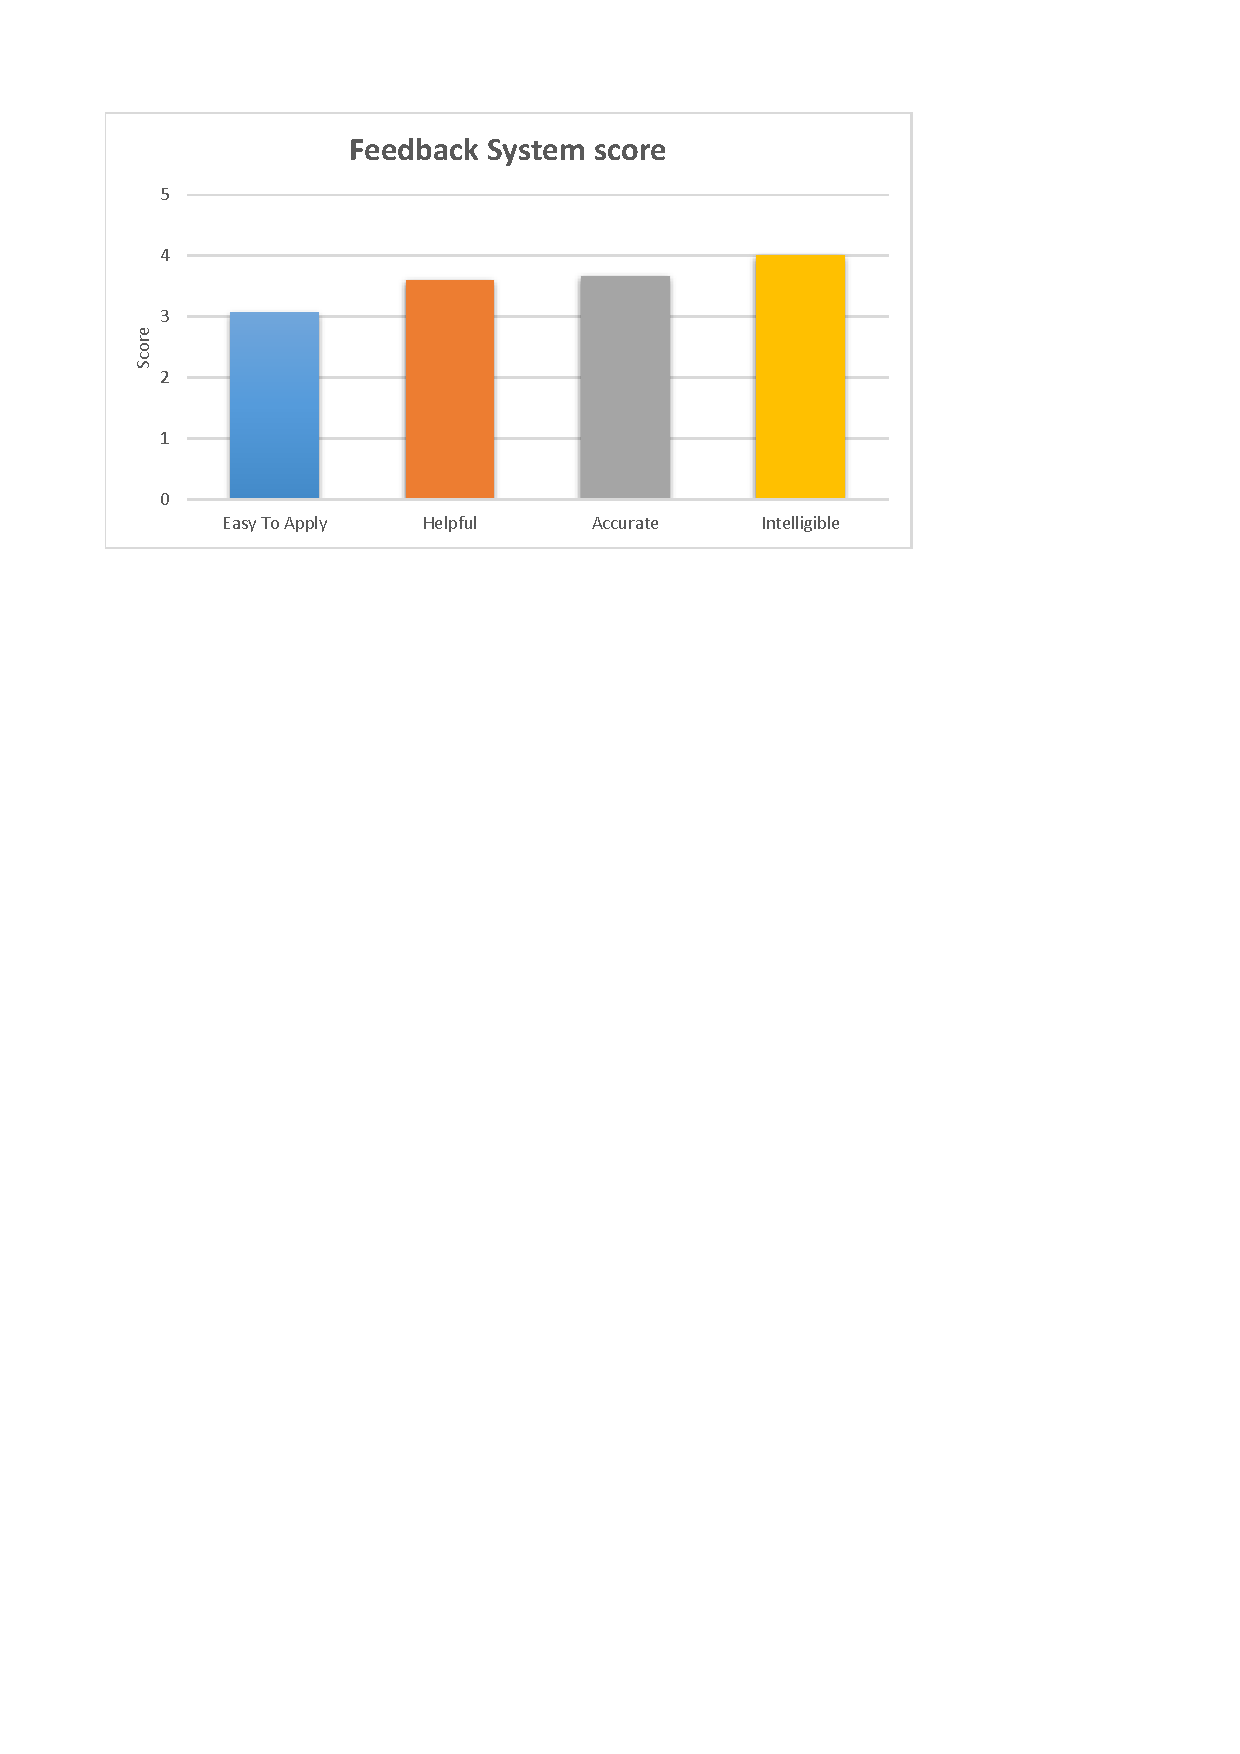
\includegraphics[width=\textwidth]{charts/feedbacksystemfeedback.pdf}
	\caption[Participants' Feedback]{Participants' Feedback}
	\label{fig:chart-feedbacksystemfeedback}
\end{figure}

\section{Discussion}
\label{sec:eval-Discussion}
From the responses in the $2^{nd}$ questionnaire, the rig setup has been well received, with participants enjoying the driving and awarding it a high score in terms of realism (see Figure \ref{fig:chart-realistic}). This suggests that is it possible to achieve a good level of realism using simple off-the-shelf hardware. 

Both groups show a noticeable improvement from one session to the next, except for the final session in which the shorter time slot allocated might have put additional pressure on the participants, hindering their performance.

For the second session, the tests shown no statistical differences in the performance of the two groups, albeit this changed for the third session. The lower average lap time for the feedback group suggests that after familiarising with the feedback system, the group started following its instructions more closely, thus improving their performance.

The available sample of participants is too small to test for correlation between gaming experience and lap times, as only three players have played sim racing games, while players of racing games among the rest have at most played arcade racing games (a simplified, non-realistic form of racing game). The same argument can be made for a possible correlation between holding a driving licence and driving performance, since all but two participants are in possession of a driving licence.
%
%Furthermore there was not statistical difference during the second session, but during the third session there was. The fact that the feedback group had a lower average lap time it suggest the group managed to get used to the feedback system after the second session and start to follow the feedback instructions during the third session. Lastly the sample is too simple to test for correlation between gaming experience and lap times, as only two players have played sim racing games while the other gamers don't play enough racing games. Same goes for correlation between having a driving licences and being able to the user the rig, as only two unlicensed participants took part, both of which are in the process of obtaining their driving license.

\section{Summary}
This chapter has presented the experiment setup, and the ensuing experiment results. Finally, a discussion is provided which argues that the feedback model implemented in \methodname is a viable solution for training race drivers using a serious games environment, in this case, a racing simulation game extended with a telemetry-based feedback system. An unexpected result is the regression participants make when the feedback system is disabled, which seems to suggest that some participants cannot cognitively retain the hints given by the feedback system, although not enough data is available to give the reason behind this. The discussion also shows that the novel method presented in this work possesses the potential to be explored further. 

%
%This chapter mainly focuses statistical tests carried out on the groups' lap times. From these test it was noted that the groups shared similar distributions and that performance of the groups is nearly identical expect for the third session. The chapter concludes by drawing claims from the tests' results. These claims state that \methodname is a valid solution which should be explored further.